\documentclass[3p]{elsarticle}
\bibliographystyle{plainnat}
\usepackage{lineno,hyperref}
\usepackage{subcaption}
\usepackage{amsmath}
\usepackage{forest}
\usepackage{courier}
\usetikzlibrary{shapes,arrows,positioning,automata}

\tikzset{
  treenode/.style = {shape=rectangle, rounded corners,
                     draw, align=center,
                     top color=white,
                     bottom color=white},
  root/.style     = {treenode, font=\Large,
                     bottom color=red!30},
  env/.style      = {treenode, font=\ttfamily\normalsize},
  dummy/.style    = {circle,draw}
}
\usepackage{caption}
\usepackage{threeparttable}
\usepackage{algorithm,algpseudocode}
\usepackage[usestackEOL]{stackengine}
\usepackage{xcolor}
\edef\tmp{\the\baselineskip}
\setstackgap{L}{\tmp}
\modulolinenumbers[1]
\linespread{1}

\journal{N/A}

\bibliographystyle{elsarticle-num}
%%%%%%%%%%%%%%%%%%%%%%%

\begin{document}

\begin{frontmatter}

\title{Governing equations and weak forms for seismic fluid-structure interaction}

% \author[A1,A2]{Somayajulu L. N. Dhulipala\corref{mycorrespondingauthor}}
% \address[A1]{Postdoctoral Research Associate, Idaho National Laboratory, Idaho Falls, ID 83402, USA}\cortext[mycorrespondingauthor]{Corresponding author; email: lakshd5@vt.edu}

\begin{abstract}
This document provides an overview of the governing equations for seismic fluid-structure interaction (FSI). The governing equation and weak form for the fluid modeling as acoustic elements is first discussed. Then, the governing equations and weak forms for the structure are presented. Finally, an interface kernel is discussed that combines the fluid and structural domain.
\end{abstract}

% \begin{keyword}
% \end{keyword}

\end{frontmatter}

% \linenumbers

\section{Acoustic fluid domain}

\noindent The following assumptions are made:
\begin{itemize}
    \item The fluid is inviscid.
    \item The fluid is irroational.
    \item The fluid is subjected to small displacements.
    \item There is no addition or subtraction of fluid.
\end{itemize}

\noindent The momentum equation is given by:
\begin{equation}
    \label{eqn:Fluid_Momentum}
    \rho_o \frac{\partial^2 \mathbf{u}_f}{\partial t^2}+\nabla p = \rho_o\mathbf{g}
\end{equation}
\noindent where $\rho_o$ is the static fluid density, $\mathbf{u}_f$ is the fluid displacement vector, $p$ is the scalar pressure, and $\mathbf{g}$ is the gravity vector with one non-zero component which is the acceleration due to gravity in the vertical direction. The continuity equation assuming there is no net mass inflow or outflow is given by:
\begin{equation}
    \label{eqn:Fluid_Continuity}
    \frac{\partial \rho_f}{\partial t}+\rho_o \nabla \cdot \frac{\partial \mathbf{u}_f}{\partial t} = 0
\end{equation}
\noindent where $\rho_f$ is the variable fluid density that is a function of time. The constitutive law is given by:
\begin{equation}
    \label{eqn:Fluid_Constitutive}
    p = c_o^2 \rho_f
\end{equation}
\noindent where $c_o$ is the speed of sound. Substituting the constitutive law in equation \eqref{eqn:Fluid_Continuity} and taking a derivative with time:
\begin{equation}
    \label{eqn:Fluid_1}
    \frac{1}{c_o^2} \frac{\partial^2 p}{\partial t^2} + \rho_o \nabla \cdot \frac{\partial^2 \mathbf{u}_f}{\partial t^2} = 0
\end{equation}

\noindent Substituting equation \eqref{eqn:Fluid_Momentum} in equation \eqref{eqn:Fluid_1}:
\begin{equation}
    \label{eqn:Fluid_2}
    \frac{1}{c_o^2} \frac{\partial^2 p}{\partial t^2} + \rho_o \nabla \cdot \Big(\mathbf{g}-\frac{1}{\rho_o} \nabla p\Big) = 0
\end{equation}

\noindent The resulting governing equation is given by:
\begin{equation}
    \label{eqn:Fluid_3}
    \frac{\partial^2 p}{\partial t^2} - c_o^2 \nabla^2p + \rho_o c_o^2 \nabla \cdot \mathbf{g} = 0
\end{equation}

\subsection{Weak form and finite element approximation}
\vspace{0.2in}
\noindent Multiplying equation \eqref{eqn:Fluid_3} with a test function $\nu_f$ and integrating over the fluid domain:

\begin{equation}
    \label{eqn:Fluid_4}
    \int_{\Omega_f} \Big(\nu_f~\frac{\partial^2 p}{\partial t^2} - \nu_f~ c_o^2~\nabla^2p + \nu_f~\rho_o c_o^2~\nabla \cdot \mathbf{g}\Big) dV = 0
\end{equation}

\noindent Using the Green's theorem, the weak form is given by:
\begin{equation}
    \label{eqn:Fluid_5}
    \int_{\Omega_f} \nu_f~\frac{\partial^2 p}{\partial t^2}~dV + c_o^2 \int_{\Omega_f} \nabla \nu_f \cdot \nabla p~dV = c_o^2 \int_{\Gamma_f} \nu_f \nabla p \cdot \mathbf{n}_f~dA - \rho_o c_o^2 \int_{\Omega_f} \nu_f~\nabla \cdot \mathbf{g}~dV
\end{equation}

\noindent The finite element approximations are given by:
\begin{equation}
    \label{eqn:Fluid_6}
    p = \mathbf{N}_f \mathbf{p}_f;~~\nu_f = \mathbf{N}_f \mathbf{c}_f
\end{equation}
\noindent where $\mathbf{N}_f$ is the shape function vector as a function of space, $\mathbf{p}_f$ is the pressure vector at the nodal points, and $\mathbf{c}_f$ is the nodal weights. Introducing the finite element approximation into equation \eqref{eqn:Fluid_5}: 
\begin{equation}
    \label{eqn:Fluid_7}
    \int_{\Omega_f} \mathbf{N}_f^T~\mathbf{N}_f~dV~\mathbf{\ddot{p}}_f + c_o^2 \int_{\Omega_f} (\nabla \mathbf{N}_f)^T \nabla \mathbf{N}_f~dV~\mathbf{{p}}_f = c_o^2 \int_{\Gamma_f} \mathbf{N}_f^T \nabla p \cdot \mathbf{n}_f~dA - \rho_o c_o^2 \int_{\Omega_f} \mathbf{N}_f^T~\nabla \cdot \mathbf{g}~dV
\end{equation}

\noindent This equation can be re-written in matrix form as:
\begin{equation}
    \label{eqn:Fluid_8}
    \mathbf{M}_f~\mathbf{\ddot{p}}_f + \mathbf{K}_f~\mathbf{p}_f = \mathbf{f}_s + \mathbf{f}_g
\end{equation}

\noindent where, $\mathbf{M}_f$ and $\mathbf{K}_f$ are similar to mass and stiffness matrices of a fluid, $\mathbf{f}_s$ is the force vector coming from the structure, and $\mathbf{f}_g$ is the gravity force vector. These quantities are further expanded as:
\begin{equation}
    \label{eqn:Fluid_9}
    \begin{aligned}
    &\mathbf{M}_f = \int_{\Omega_f} \mathbf{N}_f^T~\mathbf{N}_f~dV\\
    &\mathbf{K}_f = c_o^2 \int_{\Omega_f} (\nabla \mathbf{N}_f)^T \nabla \mathbf{N}_f~dV\\
    &\mathbf{f}_s = c_o^2 \int_{\Gamma_f} \mathbf{N}_f^T \nabla p \cdot \mathbf{n}_f~dA\\
    &\mathbf{f}_g = - \rho_o c_o^2 \int_{\Omega_f} \mathbf{N}_f^T~\nabla \cdot \mathbf{g}~dV\\
    \end{aligned}
\end{equation}

\subsection{Homogeneous gravity vector}
\vspace{0.2in}
\noindent In equation \eqref{eqn:Fluid_3}, there is a divergence of the gravity vector term (i.e., $\nabla \cdot \mathbf{g}$). If the gravity vector has constant values that are not a function of space, then its divergence becomes zero. Is such a case, the governing equation reduces to:

\begin{equation}
    \label{eqn:Fluid_10}
    \frac{\partial^2 p}{\partial t^2} - c_o^2 \nabla^2p = 0
\end{equation}

\noindent The finite element approximation in matrix form then becomes:

\begin{equation}
    \label{eqn:Fluid_11}
    \mathbf{M}_f~\mathbf{\ddot{p}}_f + \mathbf{K}_f~\mathbf{p}_f = \mathbf{f}_s
\end{equation}

\subsection{Re-writing the gravity term as a body force term}
\vspace{0.2in}
\noindent The term $\rho_o \mathbf{g}$ in equation \eqref{eqn:Fluid_Momentum} can be expressed as a generic body force vector $\mathbf{f}_{bf}$. Each term in this vector has the dimension force per unit volume. The governing equation can now be expressed as:

\begin{equation}
    \label{eqn:Fluid_12}
    \frac{\partial^2 p}{\partial t^2} - c_o^2 \nabla^2p + c_o^2 \nabla \cdot \mathbf{f}_{bf} = 0
\end{equation}

\noindent The finite element approximation in matrix form is now given by:

\begin{equation}
    \label{eqn:Fluid_13}
    \mathbf{M}_f~\mathbf{\ddot{p}}_f + \mathbf{K}_f~\mathbf{p}_f = \mathbf{f}_s + \mathbf{F}_{bf}
\end{equation}

\noindent where $\mathbf{F}_{bf}$ is given by:

\begin{equation}
    \label{eqn:Fluid_14}
    \mathbf{F}_{bf} = -c_o^2 \int_{\Omega_f} \mathbf{N}_f^T~\nabla \cdot \mathbf{f}_{bf}~dV
\end{equation}

\subsection{Assuming an incompressible fluid}
\vspace{0.2in}
\noindent If the density of the fluid is unchanging with time, then the time derivative of $\rho_f$ vanishes in equation \eqref{eqn:Fluid_Continuity}. Then the following holds:

\begin{equation}
    \label{eqn:Fluid_15}
    \nabla \cdot \frac{\partial \mathbf{u}_f}{\partial t} = 0 \iff \nabla \cdot \frac{\partial^2 \mathbf{u}_f}{\partial t^2} = 0
\end{equation}

\noindent The above equation implies that the fluid is incompressible. Substituting equation \eqref{eqn:Fluid_Momentum} into the above equation when gravity vector is expressed as a body force vector:

\begin{equation}
    \label{eqn:Fluid_16}
    \begin{aligned}
    &\nabla \cdot \Big(\mathbf{f}_{bf}-\nabla p\Big) = 0\\
    & \nabla^2p = \nabla \cdot \mathbf{f}_{bf} \iff c_o^2 \nabla^2p = c_o^2~\nabla \cdot \mathbf{f}_{bf}\\
    \end{aligned} 
\end{equation}

\noindent It is evident from the above equation that if the body force vector does not change with the spatial dimension, then its divergence equals zero. Consequently, $\nabla^2p = 0$, which is a diffusion equation. The weak form for equation \eqref{eqn:Fluid_16} is given by:

\begin{equation}
    \label{eqn:Fluid_17}
    c_o^2 \int_{\Omega_f} \nabla \nu_f \cdot \nabla p~dV = c_o^2 \int_{\Gamma_f} \nu_f \nabla p \cdot \mathbf{n}_f~dA - c_o^2 \int_{\Omega_f} \nu_f~\nabla \cdot \mathbf{f}_{bf}~dV
\end{equation}

\noindent Introducing the finite element approximation:

\begin{equation}
    \label{eqn:Fluid_18}
     c_o^2 \int_{\Omega_f} (\nabla \mathbf{N}_f)^T \nabla \mathbf{N}_f~dV~\mathbf{{p}}_f = c_o^2 \int_{\Gamma_f} \mathbf{N}_f^T \nabla p \cdot \mathbf{n}_f~dA - c_o^2 \int_{\Omega_f} \mathbf{N}_f^T~\nabla \cdot \mathbf{f}_{bf}~dV
\end{equation}

\noindent The finite element approximation in matrix form is given by:

\begin{equation}
    \label{eqn:Fluid_19}
    \mathbf{K}_f~\mathbf{p}_f = \mathbf{f}_s + \mathbf{F}_{bf}
\end{equation}

\section{Linear elastic structural domain}

\noindent The governing equation is given by:

\begin{equation}
    \label{eqn:Str_1}
    \widetilde{\nabla}^T \pmb{\sigma}_s + \mathbf{f}_{bs} = \rho_s~\frac{\partial^2\mathbf{u}_s}{\partial t^2}
\end{equation}

\noindent $\pmb{\sigma}_s$ is the Cauchy stress tensor in Voigt notation, $\mathbf{f}_{bs}$ is the body force vector, $\mathbf{u}_s$ is the displacement vector. The differential operator $\widetilde{\nabla}$ in the above equation is given by:

\begin{equation}
    \label{eqn:Str_2}
    \widetilde{\nabla} = \begin{bmatrix}
\frac{\partial}{\partial x_1} & 0 & 0\\
0 & \frac{\partial}{\partial x_2} & 0\\
0 & 0 & \frac{\partial}{\partial x_3}\\
\frac{\partial}{\partial x_2} & \frac{\partial}{\partial x_1} & 0\\
\frac{\partial}{\partial x_3} & 0 & \frac{\partial}{\partial x_1}\\
0 & \frac{\partial}{\partial x_3} & \frac{\partial}{\partial x_2}\\
\end{bmatrix}
\end{equation}

\noindent The constitutive law is given by:

\begin{equation}
    \label{eqn:Str_3}
    \pmb{\sigma}_s = \mathbf{D}_s~\pmb{\varepsilon}_s
\end{equation}

\noindent where $\mathbf{D}_s$ is the elasticity tensor and $\pmb{\varepsilon}_s$ is the Cauchy strain tensor in Voigt notation. Additionally, the strain tensor can be expressed as:

\begin{equation}
    \label{eqn:Str_4}
    \pmb{\varepsilon}_s = \widetilde{\nabla}\mathbf{u}_s
\end{equation}

\noindent Multiplying equation \eqref{eqn:Str_1} with a test function vector $\pmb{\nu}_s = [\nu_1~\nu_2~\nu_3]^T$ and integrating over the domain:

\begin{equation}
    \label{eqn:Str_5}
    \int_{\Omega_s}~\pmb{\nu}_s^T~\widetilde{\nabla}^T \pmb{\sigma}_s~dV + \int_{\Omega_s}~\pmb{\nu}_s^T~\mathbf{f}_{bs}~dV = \int_{\Omega_s}~\pmb{\nu}_s^T~\rho_s~\frac{\partial^2\mathbf{u}_s}{\partial t^2}~dV
\end{equation}

\noindent Applying the Green's theorem:

\begin{equation}
    \label{eqn:Str_6}
     \int_{\Omega_s}~\pmb{\nu}_s^T~\rho_s~\frac{\partial^2\mathbf{u}_s}{\partial t^2}~dV + \int_{\Omega_s}~(\widetilde{\nabla}\pmb{\nu}_s)^T~ \pmb{\sigma}_s~dV = \int_{\Gamma_s}~\pmb{\nu}_s^T~\mathbf{t}_s~dA + \int_{\Omega_s}~\pmb{\nu}_s^T~\mathbf{f}_{bs}~dV
\end{equation}

\noindent where $\mathbf{t}_s$ is the traction vector given by:

\begin{equation}
    \label{eqn:Str_7}
     \mathbf{t}_s = \mathbf{S}_s~\mathbf{n}_s
\end{equation}

\noindent where $\mathbf{S}_s$ is the Cauchy stress tensor and $\mathbf{n}_s$ is the normal vector. The finite element approximations are given by:

\begin{equation}
    \label{eqn:Str_8}
    \mathbf{u}_s = \mathbf{N}_s\mathbf{d}_s;~\pmb{\nu}_s = \mathbf{N}_s\mathbf{c}_s
\end{equation}

\noindent where $\mathbf{N}_s$ contain the finite element shape functions, $\mathbf{d}_s$ is the nodal displacement vector, and $\mathbf{c}_s$ is the nodal weights vector. The finite element approximation is given by:

\begin{equation}
    \label{eqn:Str_9}
    \int_{\Omega_s}~\mathbf{N}_s^T~\rho_s~\mathbf{N}_s~dV~\ddot{\mathbf{d}}_s + \int_{\Omega_s}~(\widetilde{\nabla}\mathbf{N}_s)^T~ \mathbf{D}_s~\widetilde{\nabla}\mathbf{N}_s~dV~\mathbf{d}_s = \int_{\Gamma_s}~\mathbf{N}_s^T~\mathbf{t}_s~dA + \int_{\Omega_s}~\mathbf{N}_s^T~\mathbf{f}_{bs}~dV
\end{equation}

\noindent The finite element approximation can be expressed in matrix form as:

\begin{equation}
    \label{eqn:Str_10}
    \mathbf{M}_s~\ddot{\mathbf{d}}_s + \mathbf{K}_s~\mathbf{d}_s = \mathbf{f}_f + \mathbf{F}_{bs}
\end{equation}

\noindent where $\mathbf{M}_s$ and $\mathbf{K}_s$ are similar to the mass and stiffness matrices, respectively, $\mathbf{f}_f$ is the force vector coming from the fluid, and $\mathbf{F}_{bs}$ is the body force vector. These quantities are further expanded as:

\begin{equation}
    \label{eqn:Str_11}
    \begin{aligned}
    &\mathbf{M}_s = \int_{\Omega_s}~\mathbf{N}_s^T~\rho_s~\mathbf{N}_s~dV\\
    &\mathbf{K}_s = \int_{\Omega_s}~(\widetilde{\nabla}\mathbf{N}_s)^T~ \mathbf{D}_s~\widetilde{\nabla}\mathbf{N}_s~dV\\
    &\mathbf{f}_f = \int_{\Gamma_s}~\mathbf{N}_s^T~\mathbf{t}_s~dA\\
    &\mathbf{F}_{bs} = \int_{\Omega_s}~\mathbf{N}_s^T~\mathbf{f}_{bs}~dV\\
    \end{aligned}
\end{equation}

\section{Interface kernel coupling fluid and structural domains (no fluid body forces and compressible fluid)}

\noindent The boundary between the fluid and structure is denoted as $\Gamma_{sf}$. At this boundary, the displacements in the normal direction for the fluid and structural domains are the same:

\begin{equation}
    \label{eqn:Int_1}
    \mathbf{u}_s \cdot \mathbf{n} = \mathbf{u}_f \cdot \mathbf{n}
\end{equation}

\noindent where $\mathbf{n}$ is the normal vector given by $\mathbf{n} = \mathbf{n}_f = -\mathbf{n}_s$. In addition, there is continuity of pressure at the boundary as expressed by the structural Cauchy stress tensor:

\begin{equation}
\label{eqn:Int_2}
    [\mathbf{S}_s]_{\Gamma_{sf}}=-p~\mathbf{I}
\end{equation}

\noindent where $\mathbf{I}$ is an identity matrix. The structural forcing term coming from the fluid is now given by:

\begin{equation}
\label{eqn:Int_3}
    \begin{aligned}
    \mathbf{f}_f &= \int_{\Gamma_{sf}}~\mathbf{N}_s^T~\mathbf{t}_s~dA\\
    &= \int_{\Gamma_{sf}}~\mathbf{N}_s^T~\mathbf{S}_s~\mathbf{n}_s~dA\\
    &= \int_{\Gamma_{sf}}~\mathbf{N}_s^T~-p\mathbf{I}~\mathbf{n}_s~dA\\
    &= \int_{\Gamma_{sf}}~\mathbf{N}_s^T~p~\mathbf{n}~dA\\
    &= \int_{\Gamma_{sf}}~\mathbf{N}_s^T~\mathbf{n}~p~dA\\
    &= \int_{\Gamma_{sf}}~\mathbf{N}_s^T~\mathbf{n}~\mathbf{N}_f~dA~\mathbf{p}_f\\
    \end{aligned}
\end{equation}

\noindent where the relation $\mathbf{n} = -\mathbf{n}_s$ is used. Without body forces, the fluid momentum equation is given by:

\begin{equation}
\label{eqn:Int_4}
    \nabla p = -\rho_o~\frac{\partial^2\mathbf{u}_f}{\partial t^2}
\end{equation}

\noindent At the fluid-structure boundary, the fluid displacements can be expressed in terms of structural accelerations as:

\begin{equation}
\label{eqn:Int_4}
\begin{aligned}
    \mathbf{n}^T[\nabla p]_{\Gamma_{sf}} &= -\rho_o~\mathbf{n}^T~\big[\frac{\partial^2\mathbf{u}_f}{\partial t^2}\big]_{\Gamma_{sf}}\\
    &= -\rho_o~\mathbf{n}^T~\big[\frac{\partial^2\mathbf{u}_s}{\partial t^2}\big]_{\Gamma_{sf}}\\
    &= -\rho_o~\mathbf{n}^T~\big[\mathbf{N}_s~\ddot{\mathbf{d}}_s\Big]_{\Gamma_{sf}}\\
    \end{aligned}
\end{equation}

\noindent The fluid forcing vector coming from the structure is now expressed as:

\begin{equation}
    \label{eqn:Int_5}
    \begin{aligned}
    \mathbf{f}_s &= c_o^2 \int_{\Gamma_{sf}} \mathbf{N}_f^T \nabla p \cdot \mathbf{n}_f~dA\\
    &= c_o^2 \int_{\Gamma_{sf}} \mathbf{N}_f^T \nabla p \cdot \mathbf{n}~dA\\
    &= c_o^2 \int_{\Gamma_{sf}} \mathbf{N}_f^T~\mathbf{n}^T\nabla p~dA\\
    &= -\rho_oc_o^2 \int_{\Gamma_{sf}} \mathbf{N}_f^T~\mathbf{n}^T~\mathbf{N}_s~dA~\ddot{\mathbf{d}}_s\\
    \end{aligned}
\end{equation}

\noindent Introducing the interface matrix $\mathbf{H}$:

\begin{equation}
\label{eqn:Int_6}
    \mathbf{H} = \int_{\Gamma_{sf}}~\mathbf{N}_s^T~\mathbf{n}~\mathbf{N}_f~dA
\end{equation}

\noindent The structural and fluid forcing functions are given by:

\begin{equation}
\label{eqn:Int_7}
    \begin{aligned}
    &\mathbf{f}_f = \mathbf{H}\mathbf{p}_f\\
    &\mathbf{f}_s = -\rho_oc_o^2\mathbf{H}^T\mathbf{\ddot{d}}_s\\
    \end{aligned}
\end{equation}

\noindent The combined finite element equations for fluid and structural domains is:

\begin{equation}
\label{eqn:Int_8}
    \begin{bmatrix}
\mathbf{M}_s & 0\\
\rho_oc_o^2\mathbf{H}^T & \mathbf{M}_f\\
\end{bmatrix} \begin{bmatrix}
\mathbf{\ddot{d}}_s\\
\mathbf{\ddot{p}}_f\\
\end{bmatrix} + \begin{bmatrix}
\mathbf{K}_s & -\mathbf{H}\\
0 & \mathbf{K}_f\\
\end{bmatrix} \begin{bmatrix}
\mathbf{{d}}_s\\
\mathbf{{p}}_f\\
\end{bmatrix} = \begin{bmatrix}
\mathbf{F}_{bs}\\
\mathbf{0}_f\\
\end{bmatrix}
\end{equation}

\noindent where $\mathbf{0}_f$ is a vector of zeros.

\section{Summary of the fluid and structural domains finite element equations}

\noindent The structural domain finite element equation in matrix form is:

\begin{equation}
    \label{eqn:summ_1}
    \mathbf{M}_s~\mathbf{\ddot{d}}_s + \mathbf{K}_s~\mathbf{d}_s - \mathbf{H}~\mathbf{p}_f = \mathbf{F}_{bs}
\end{equation}

\noindent The different terms in the above equation are expanded below:

\begin{itemize}
    \item $\mathbf{M}_s = \int_{\Omega_s}~\mathbf{N}_s^T~\rho_s~\mathbf{N}_s~dV$ is the structural mass matrix which integrates over the density of the structural domain.
    \item $\mathbf{K}_s = \int_{\Omega_s}~(\widetilde{\nabla}\mathbf{N}_s)^T~ \mathbf{D}_s~\widetilde{\nabla}\mathbf{N}_s~dV$ is the structural stiffness matrix which integrates over the elasticity tensor of the structural domain.
    \item $\mathbf{H} = \int_{\Gamma_{sf}}~\mathbf{N}_s^T~\mathbf{n}~\mathbf{N}_f~dA$ is the interface matrix which transfers the displacements from structure to fluid and pressures from fluid to structure.
    \item $\mathbf{F}_{bs} = \int_{\Omega_s}~\mathbf{N}_s^T~\mathbf{f}_{bs}~dV$ is the structural body force vector.
    \item $\mathbf{d}_s$ is the structural displacement vector at the nodes in the finite-element mesh.
    \item $\mathbf{p}_f$ is the pressure vector at the nodes.
\end{itemize}

\noindent The fluid domain finite element equation in matrix form is:

\begin{equation}
    \label{eqn:summ_2}
    \rho_o c_o^2 \mathbf{H}^T~\mathbf{\ddot{d}}_s + \mathbf{M}_f~\mathbf{\ddot{p}}_f + \mathbf{K}_f~\mathbf{p}_f = \mathbf{0}_f
\end{equation}

% &\\
%     &\\

\begin{itemize}
    \item $\rho_o$ is the static density of the fluid.
    \item $c_o$ is the speed of wave propagation through the fluid.
    \item $\mathbf{M}_f = \int_{\Omega_f} \mathbf{N}_f^T~\mathbf{N}_f~dV$ is similar to the mass matrix for the fluid domain.
    \item $\mathbf{K}_f = c_o^2 \int_{\Omega_f} (\nabla \mathbf{N}_f)^T \nabla \mathbf{N}_f~dV$ is similar to the stiffness matrix for the fluid domain.
    \item $\mathbf{0}_f$ is a vector of zeros.
\end{itemize}

\section{Equivalence between acoustic and structural mechanics governing equations}

\noindent Consider a structural domain. If the displacements in two directions are zero everywhere in the domain, one governing equation is sufficient to describe the domain behavior:

\begin{equation}
    \label{eqn:Eql_Struc1}
    \frac{\lambda^e + 2 G^e}{G^e}\frac{\partial^2u_{s,1}^e}{\partial x_1^2}+\frac{\partial^2u_{s,1}^e}{\partial x_2^2}+\frac{\partial^2u_{s,1}^e}{\partial x_3^2} = \frac{\rho^e}{G^e}~\frac{\partial^2u_{s,1}^e}{\partial t^2}
\end{equation}

\noindent where, the superscript indicates a structural domain that is equivalent to the acoustic domain, and $\lambda$, $G$, and $\rho$ are the Lam\'e's constant, shear modulus, and density, respectively. The above equation assumes that the equivalent structural domain has no body force. Further, if we set $\lambda^e = -G^e$ in the above equation:

\begin{equation}
    \label{eqn:Eql_Struc2}
    \frac{\partial^2u_{s,1}^e}{\partial x_1^2}+\frac{\partial^2u_{s,1}^e}{\partial x_2^2}+\frac{\partial^2u_{s,1}^e}{\partial x_3^2} = \frac{\rho^e}{G^e}~\frac{\partial^2u_{s,1}^e}{\partial t^2}
\end{equation}

\noindent Now, expanding the acoustic domain governing equation [equation \eqref{eqn:Fluid_10}]:

\begin{equation}
    \label{eqn:Eql_Struc3}
    \frac{\partial^2 p}{\partial x_1^2}+\frac{\partial^2 p}{\partial x_2^2}+\frac{\partial^2 p}{\partial x_3^2} = \frac{1}{c_o^2}~\frac{\partial^2 p}{\partial t^2}
\end{equation}

\noindent We see that equations \eqref{eqn:Eql_Struc2} and \eqref{eqn:Eql_Struc3} are equivalent if $\rho^e = \frac{G^e}{c_o^2}$, $\lambda^e = -G^e$, and Young's modulus $E^e \to +\infty$.

\section{Implementing acoustics and equivalent structural mechanics approaches in MASTODON}

\noindent The equivalence between acoustics and structural mechanics governing equations is presented below:

\begin{equation}
    \label{eqn:Ac_Mech_Eq1}
    \begin{aligned}
        &\nabla^2p = \frac{1}{c_o^2}\frac{\partial^2p}{\partial t^2} \iff \nabla^2u^e_{s,1} = \frac{\rho^e}{G^e}\frac{\partial^2u^e_{s,1}}{\partial t^2}\\
       &\textrm{such that,}~\rho^e = \frac{G^e}{c_o^2}~\textrm{and}~\lambda^e = -G^e\\
    \end{aligned}
\end{equation}

\noindent In MASTODON, the acoustics approach is implemented by using the \texttt{Diffusion} kernel for the $\nabla^2p$ term and the \texttt{InertialForce} kernel with density $\frac{1}{c_o^2}$ for the $\frac{\partial^2p}{\partial t^2}$ term in equation \eqref{eqn:Ac_Mech_Eq1}. The equivalent structural mechanics approach is implemented by using the \texttt{DynamicTensorMechanics} kernel for the $\nabla^2u^e_{s,1}$ term and the \texttt{InertialForce} kernel with density $\frac{G^e}{c_o^2}$ for the $\frac{\partial^2u^e_{s,1}}{\partial t^2}$ term in equation \eqref{eqn:Ac_Mech_Eq1}. Furthermore, the \texttt{ComputeIsotropicElasticityTensor} material is used for the structural mechanics approach with material parameters defined as per the second line of equation \eqref{eqn:Ac_Mech_Eq1}. It is noted that $G^e$ can be set to any arbitrary value.

\subsection{Finite element mesh}

\noindent Figure \ref{fig:Mesh} presents the mesh for performing the simulations. It is a 2D mesh with a time varying pressure boundary (Dirichlet) condition applied at the bottom edge. Pressure is recorded at the middle of the top edge. Also, for the equivalent structural mechanics approach, the displacements in the y-direction are constrained to zero along the four edges and the pressure boundary condition is equivalent to applying a displacement in the x-direction at the bottom edge.

\begin{figure}[H]
\centering
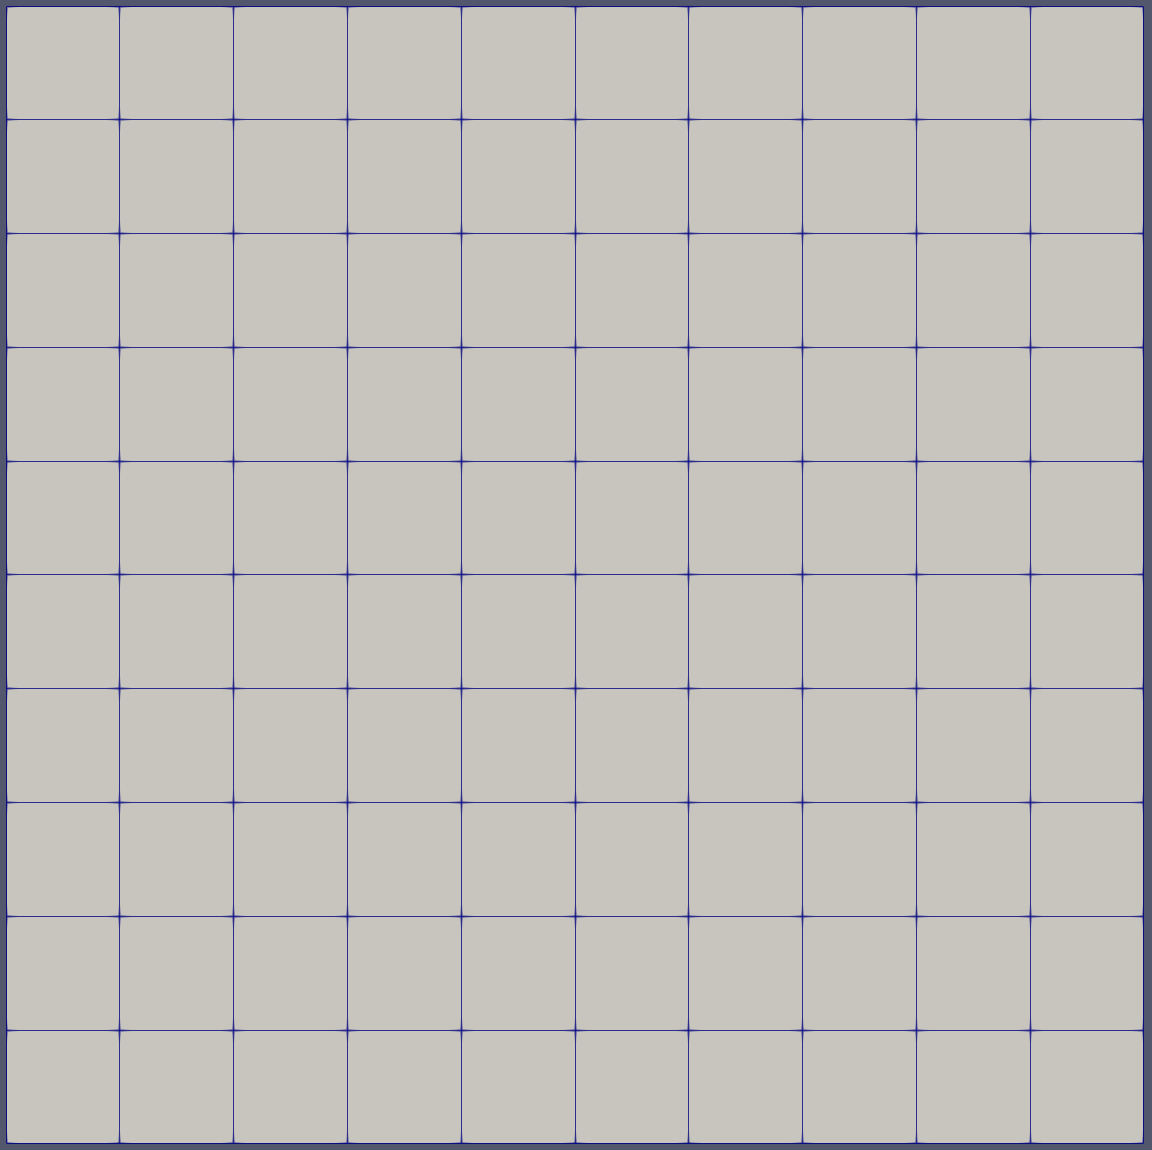
\includegraphics[width=3in, height=2.5in]{Mesh.png} 
\caption{A 2D mesh for simulating acoustics.}
\label{fig:Mesh}
\end{figure}

\subsection{Results}

\noindent The input pressure at the bottom edge of the mesh is presented in Figure \ref{fig:Input}. Figure \ref{fig:Comparison} presents the pressures at the center of the top edge for the acoustics and equivalent structural mechanics approaches considering three $c_o^2$ values: $1~m/s$, $200~m/s$, and $1450~m/s$. It is seen that the results using the two approaches are identical. 

\begin{figure}[H]
\centering
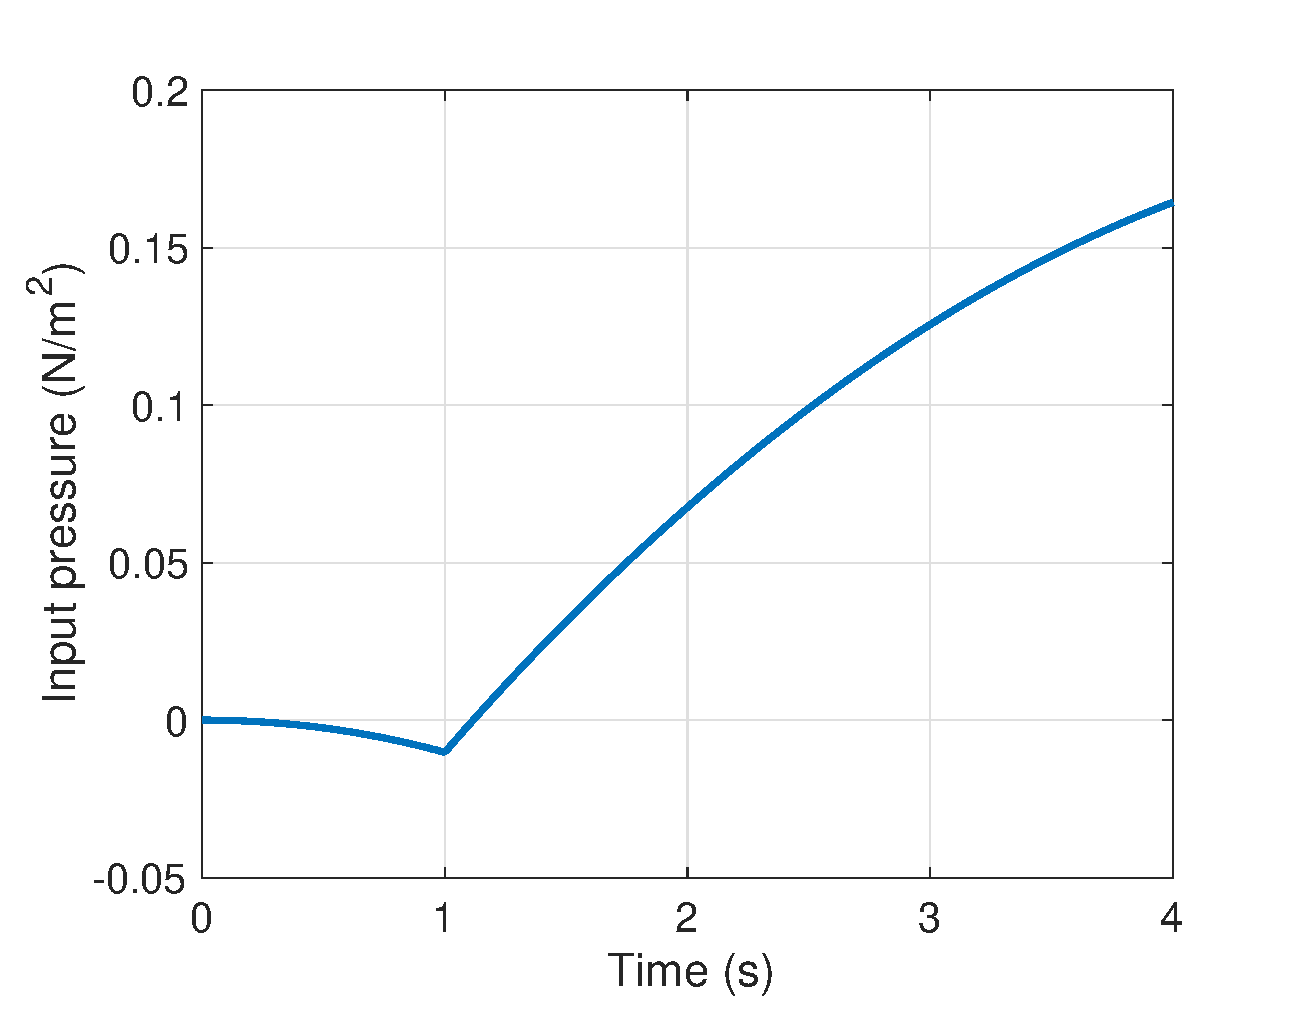
\includegraphics[width=3in, height=2.5in]{Input.eps} 
\caption{Input pressure at the bottom edge of the mesh.}
\label{fig:Input}
\end{figure}

\begin{figure}[H]
\begin{subfigure}{0.5\textwidth}
\centering
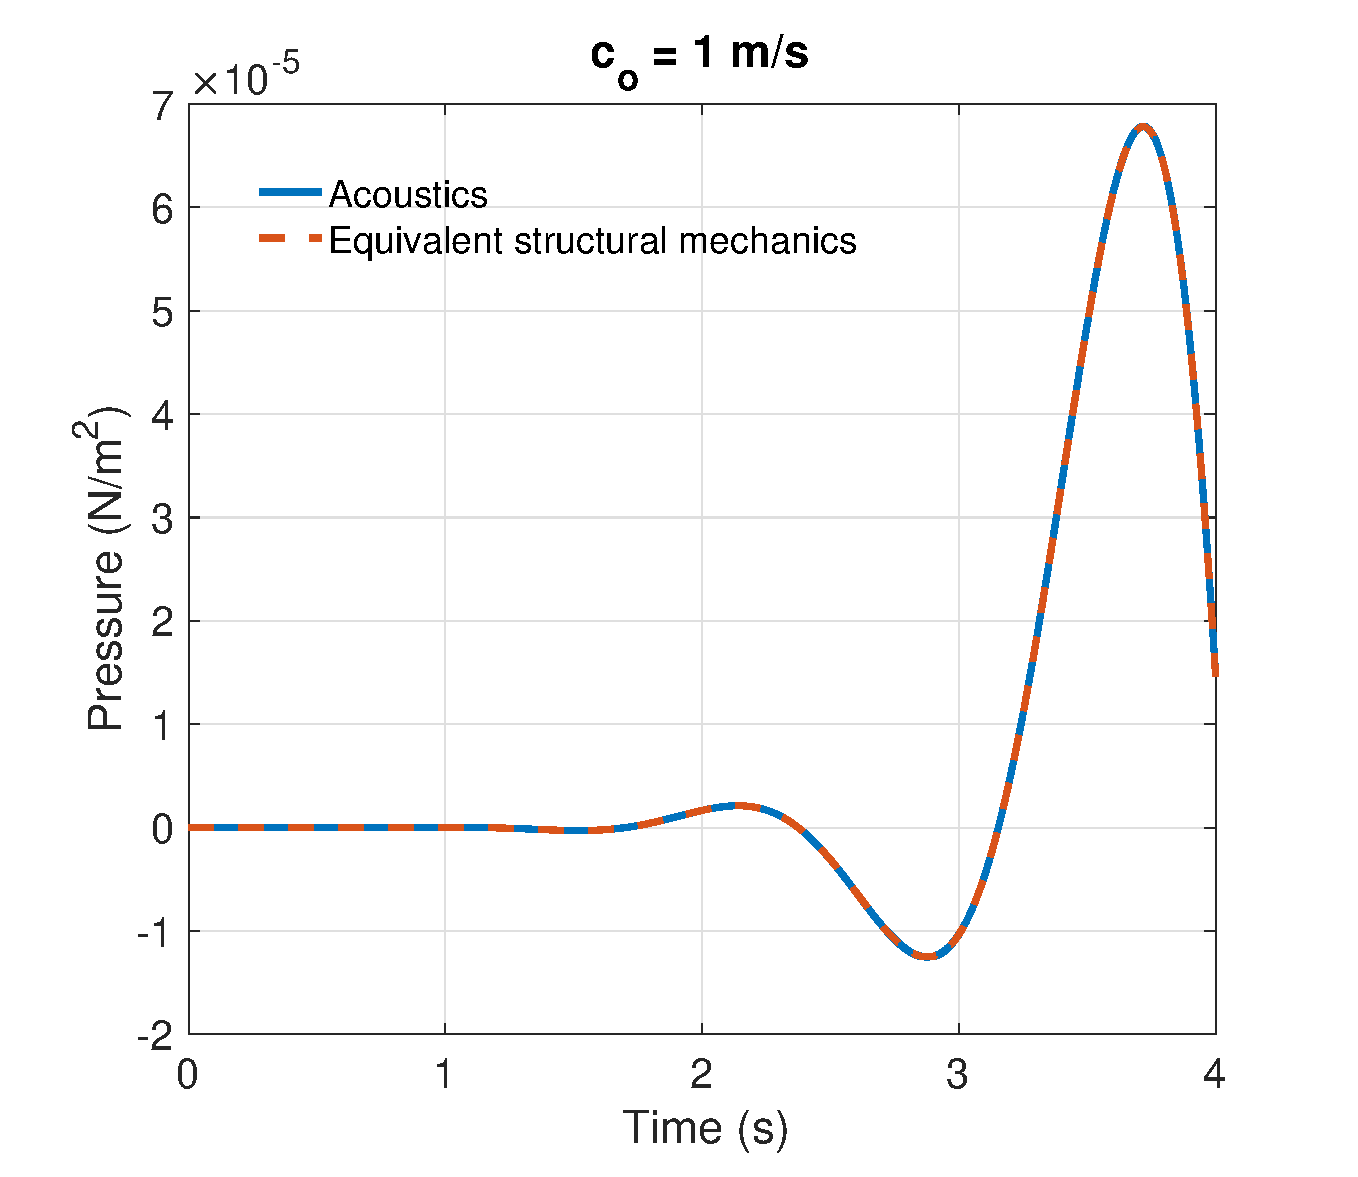
\includegraphics[width=2.5in, height=2.1in]{C_1.eps} 
\caption{}
\label{fig:C1}
\end{subfigure}
\begin{subfigure}{0.5\textwidth}
\centering
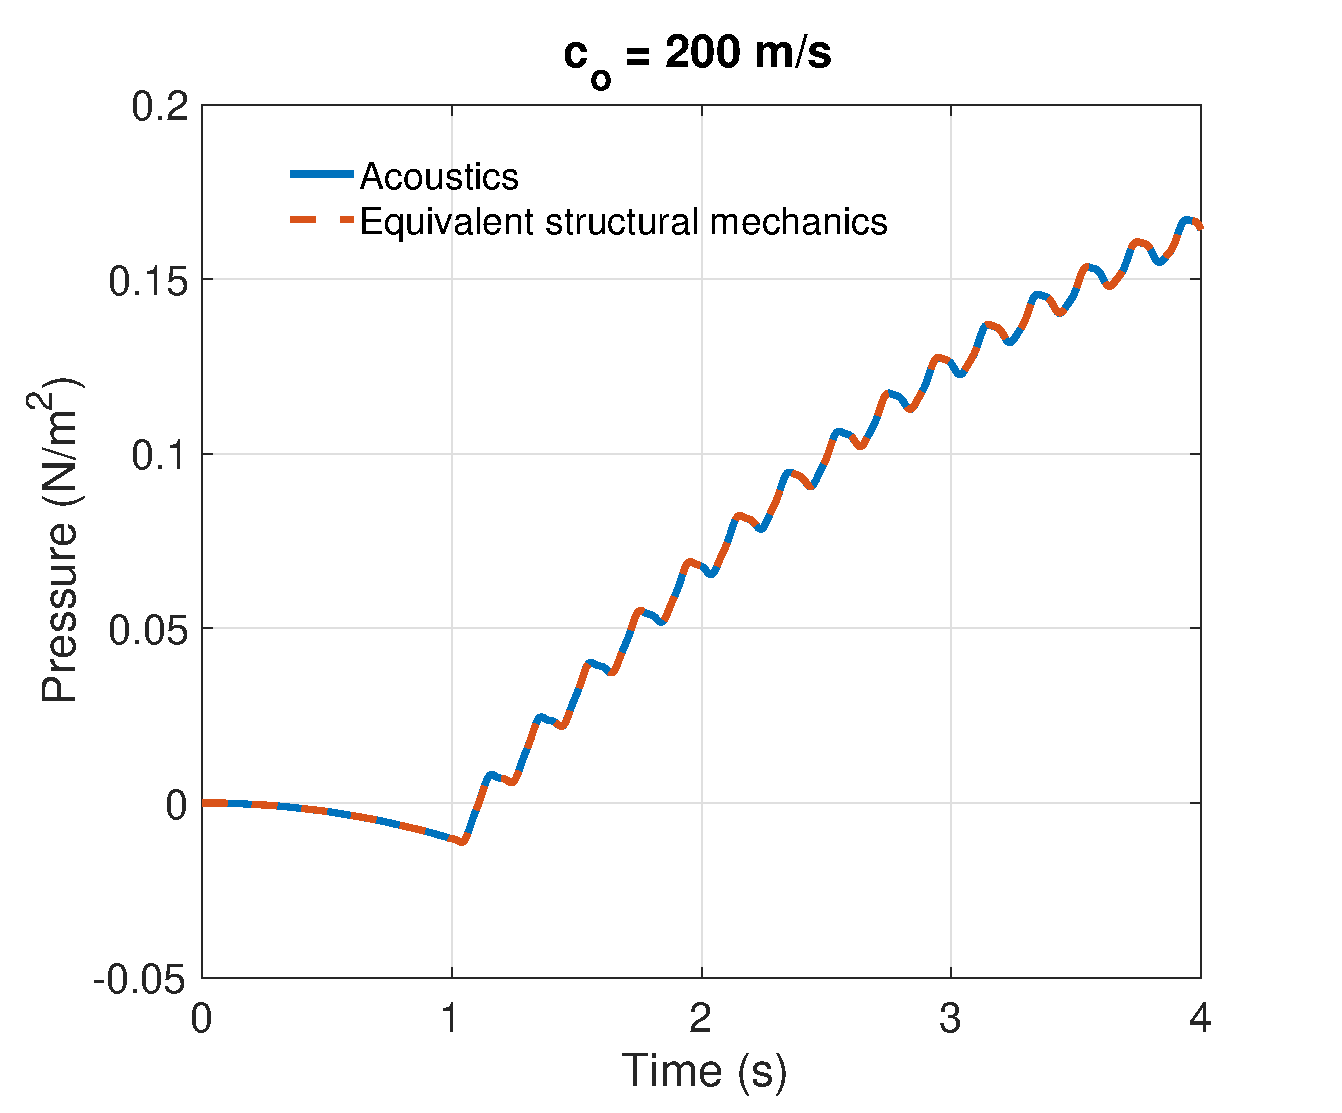
\includegraphics[width=2.5in, height=2.1in]{C_200.eps} 
\caption{}
\label{fig:C200}
\end{subfigure}
\begin{subfigure}{1\textwidth}
\centering
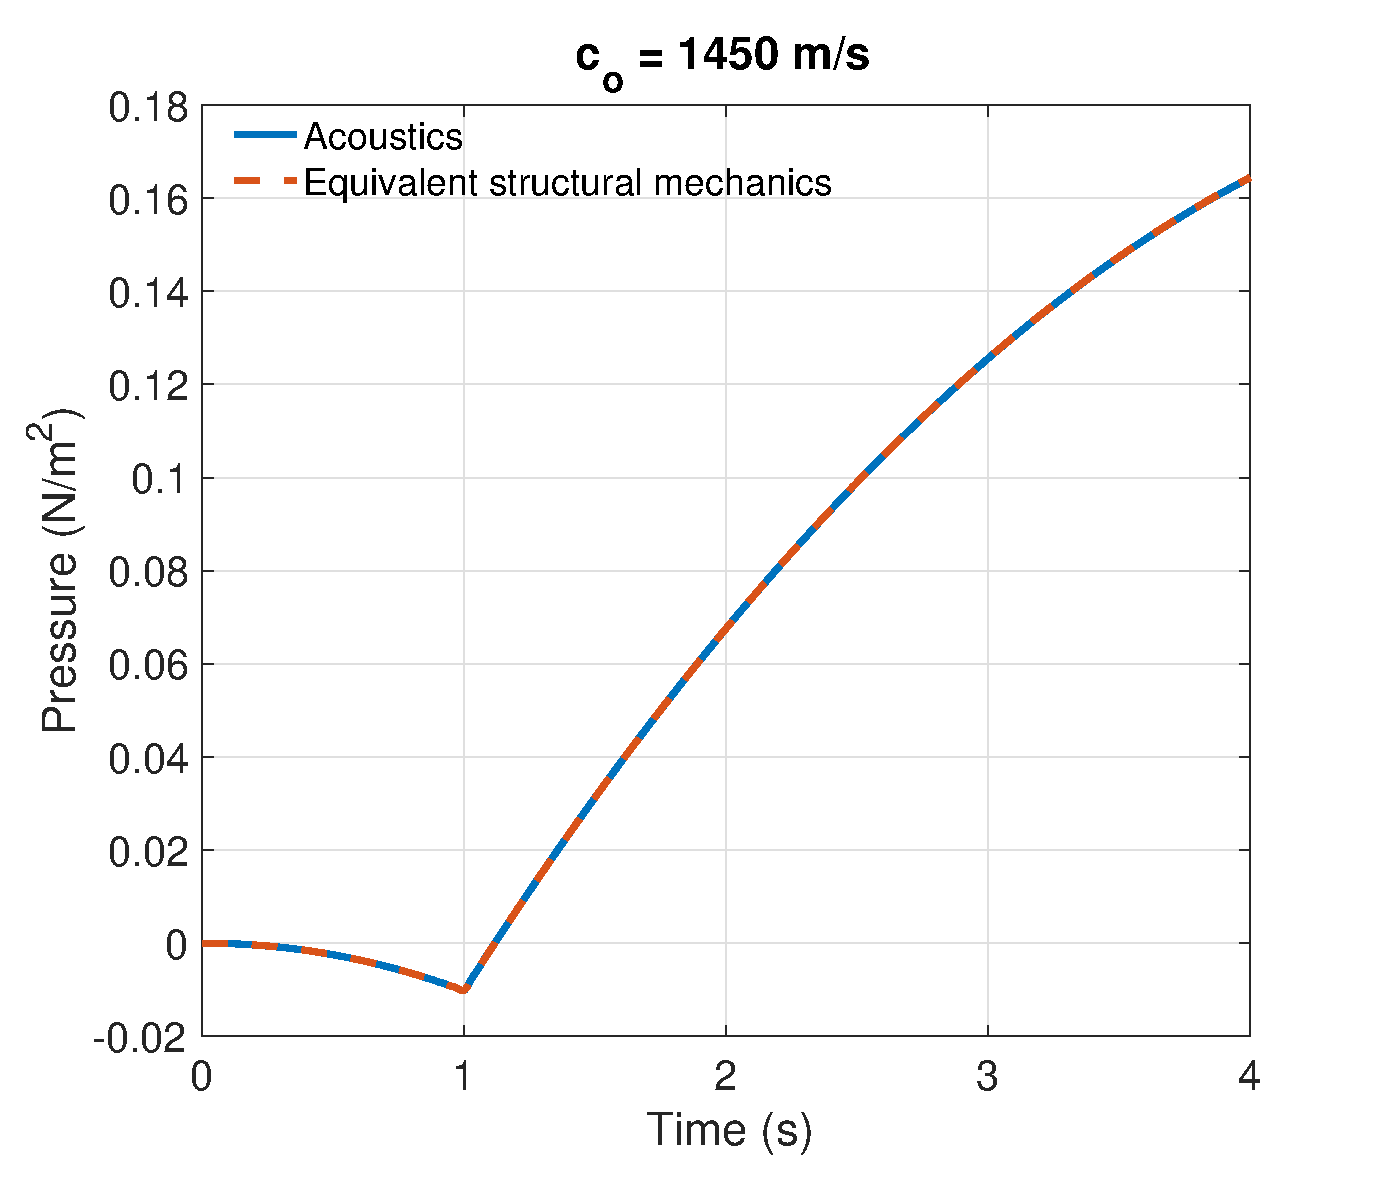
\includegraphics[width=2.5in, height=2.1in]{C_1450.eps} 
\caption{}
\label{fig:C1450}
\end{subfigure}
\caption{Comparison between acoustics and equivalent structural mechanics approaches for different $c_o$ values.}
\label{fig:Comparison}
\end{figure}

\noindent Figure \ref{fig:XY_dir} presents the distribution of x-direction displacements (i.e., pressure) and y-direction dummy displacements in the equivalent structural mechanics mesh. It is seen that the y-direction dummy displacements are very close to zero.

\begin{figure}[H]
\begin{subfigure}{1\textwidth}
\centering
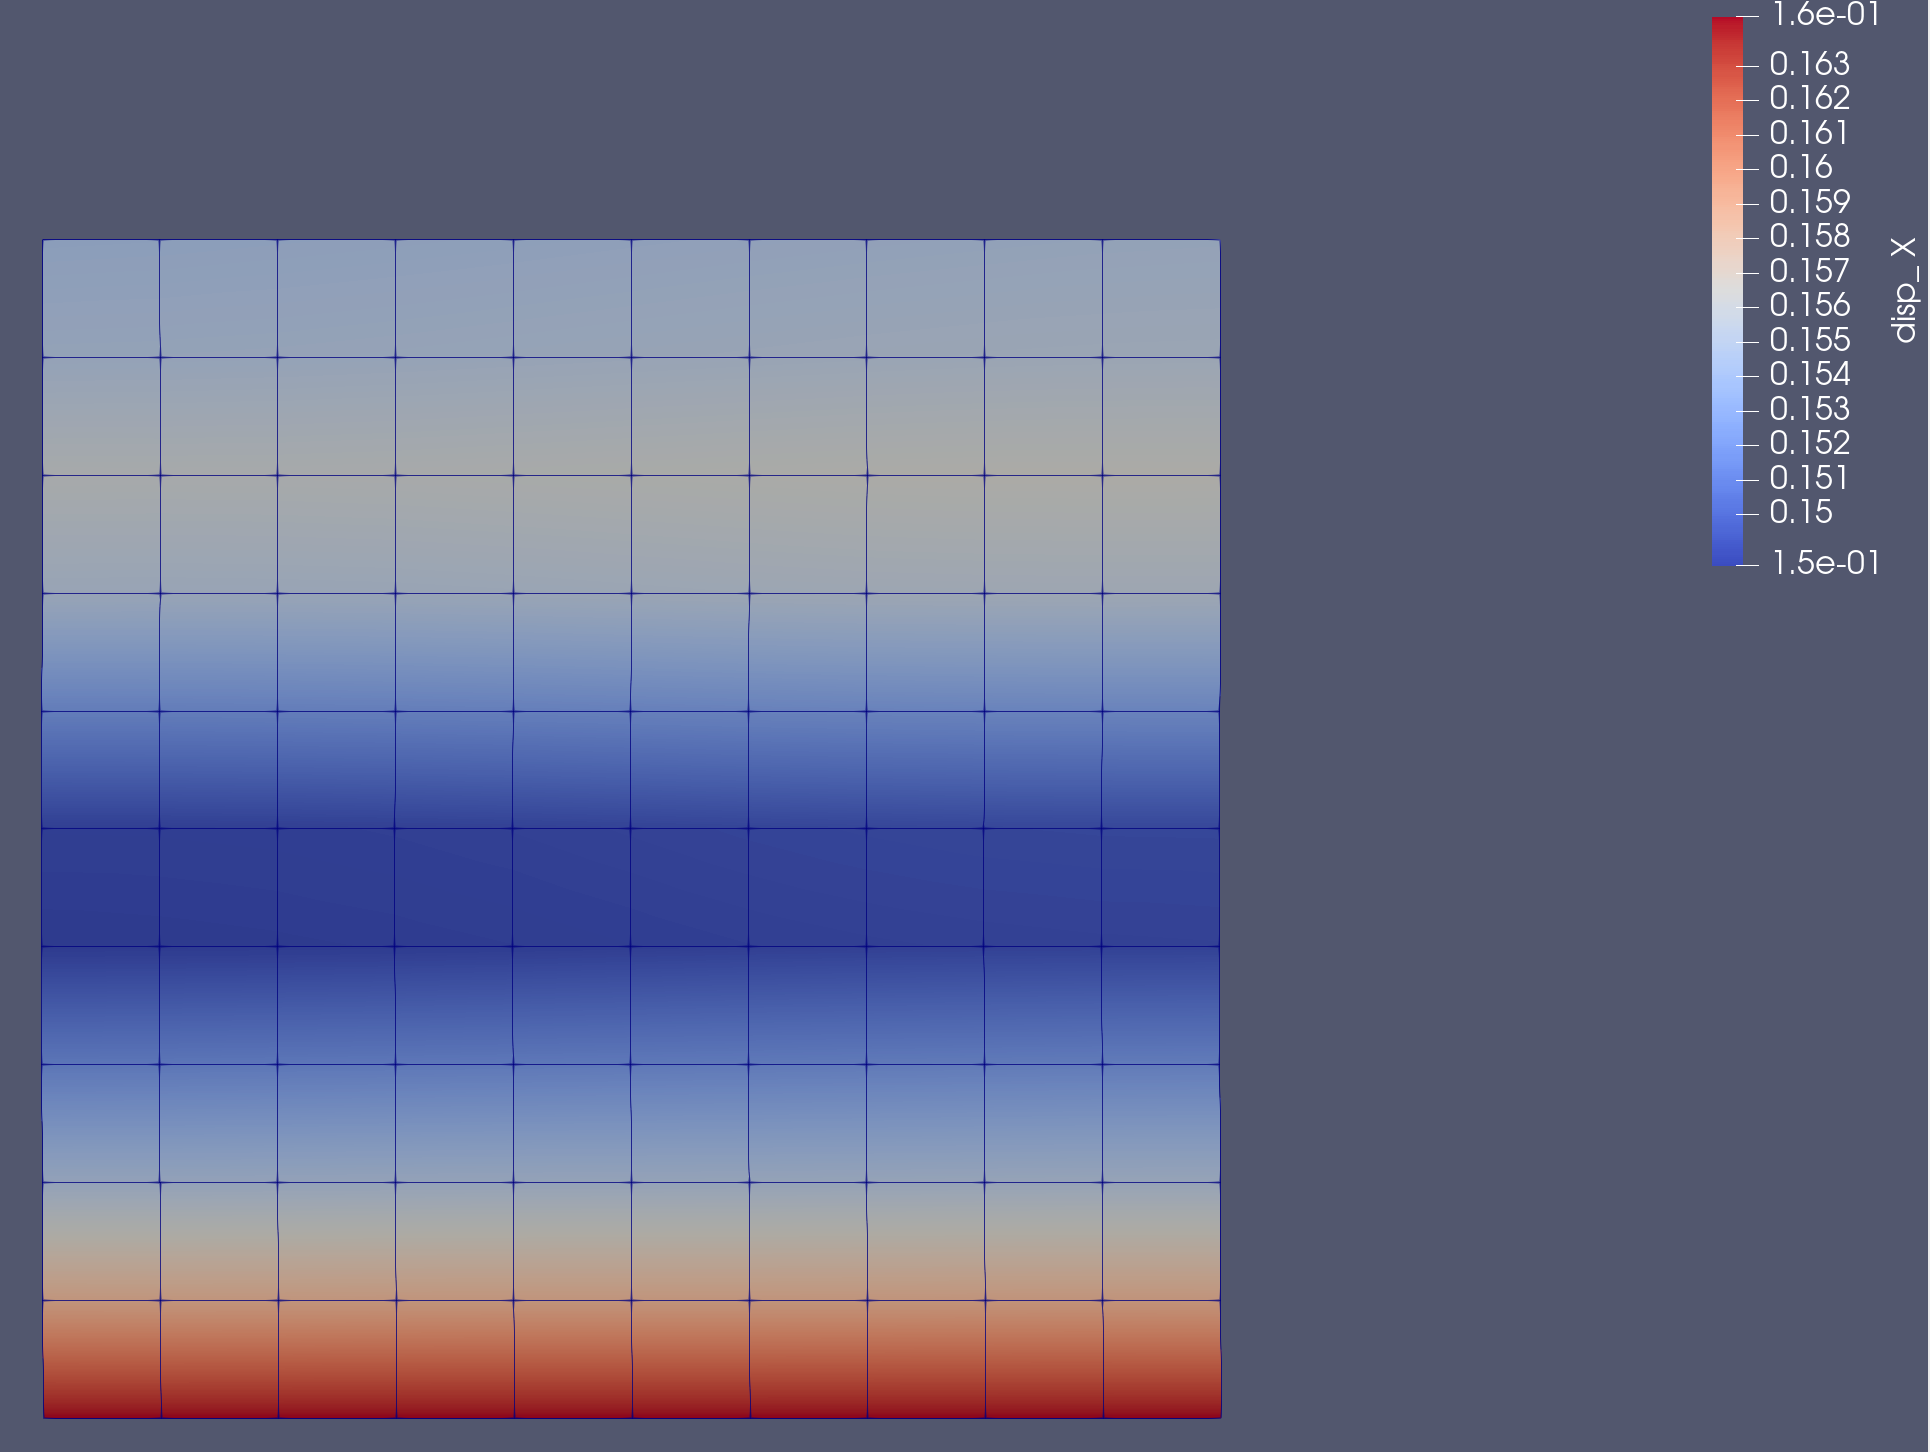
\includegraphics[width=3in, height=2.5in]{disp_X_eqstr_C200.png} 
\caption{}
\label{fig:X_dir}
\end{subfigure}
\begin{subfigure}{1\textwidth}
\centering
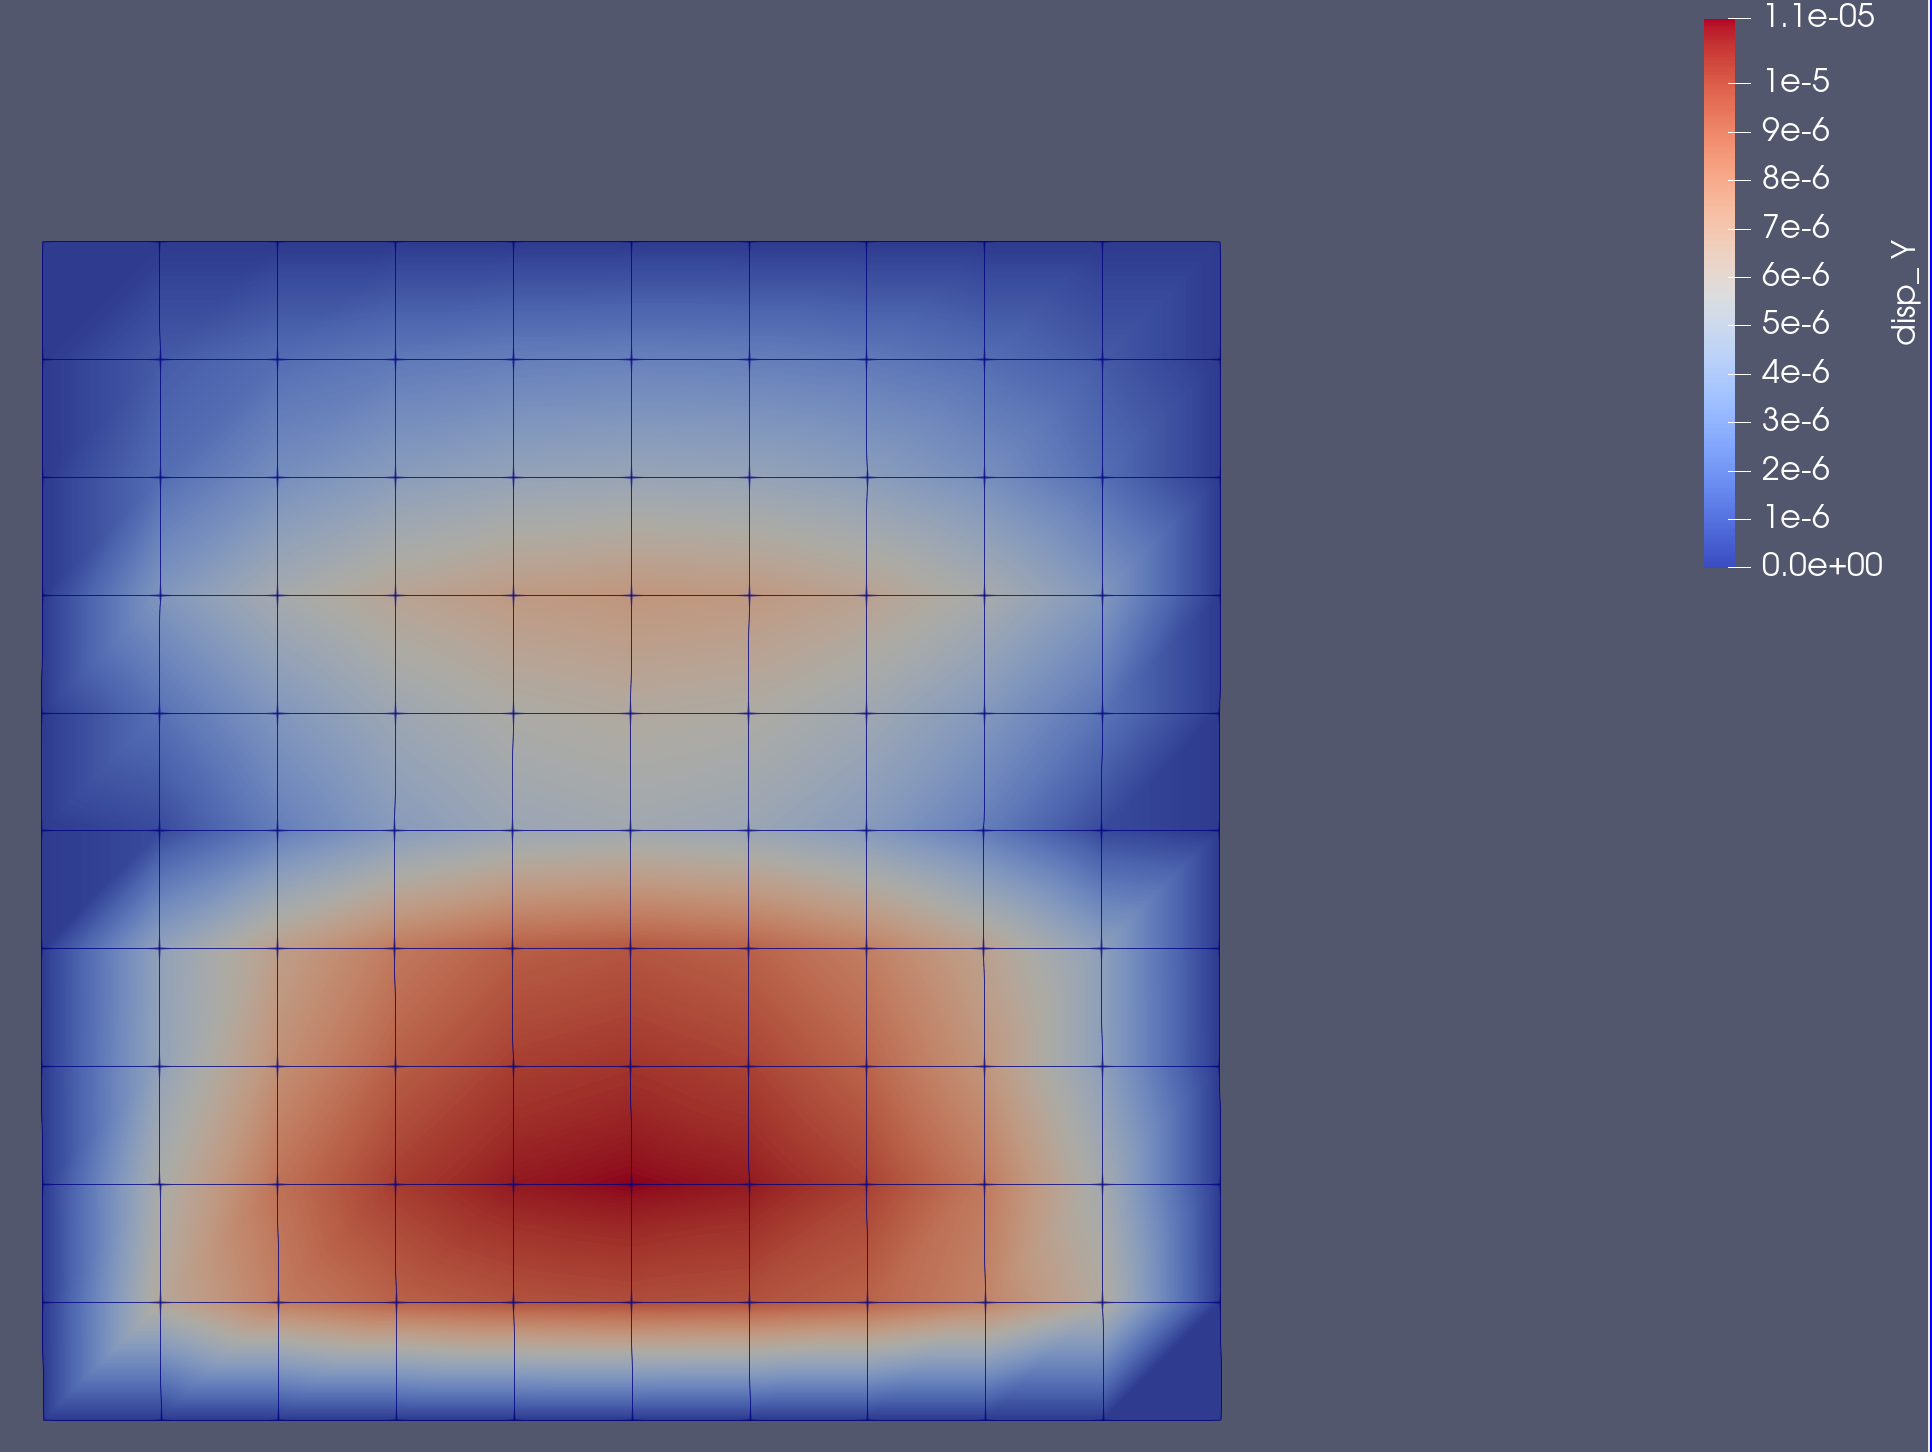
\includegraphics[width=3in, height=2.5in]{disp_Y_eqstr_C200.png} 
\caption{}
\label{fig:Y_dir}
\end{subfigure}
\caption{Distribution of (a) x-direction displacements (i.e., pressure) and (b) y-direction dummy displacements in the equivalent structural mechanics mesh.)}
\label{fig:XY_dir}
\end{figure}

% \begin{figure}
% \begin{subfigure}{0.5\textwidth}
% \centering
% \includegraphics[width=3in, height=2.5in]{M_R.eps} 
% \caption{}
% \label{fig:Mesh}
% \end{subfigure}
% \begin{subfigure}{0.5\textwidth}
% \centering
% \includegraphics[width=3in, height=2.5in]{Response_Spectrum.eps} 
% \caption{}
% \label{fig:GM2}
% \end{subfigure}
% \caption{(a) Magnitude-distance values and (b) response spectra of the ground motions considered in this study. \textbf{\textcolor{red}{Change plot (b).}}}
% \label{fig:GM}
% \end{figure}

\begin{thebibliography}{9}
\bibitem{R1} 
Rienstra, S. W., \& Hirschberg, A. (2004). An introduction to acoustics. \textit{Eindhoven University of Technology}, 18, 19.

\bibitem{R2} 
Bathe, K. J., Nitikitpaiboon, C., \& Wang, X. (1995). A mixed displacement-based finite element formulation for acoustic fluid-structure interaction. \textit{Computers \& Structures}, 56(2-3), 225-237.

\bibitem{R3}
Wang, X., \& Bathe, K. J. (1997). Displacement/pressure based mixed finite element formulations for acoustic fluid–structure interaction problems. \textit{International journal for numerical methods in engineering}, 40(11), 2001-2017.

\bibitem{R4}
Sandberg, G., \& Ohayon, R. (Eds.). (2009). \textit{Computational aspects of structural acoustics and vibration} (Vol. 505). Springer Science \& Business Media.

\bibitem{R5}
Zhao, C., Chen, J., \& Yu, N. (2017). Dynamic response of AP1000 water tank with internal ring baffles under earthquake loads. \textit{Energy Procedia}, 127, 407-415.

\bibitem{R6}
Kohnke, P. C. (Ed.). (1999). \textit{ANSYS Theory Reference: Release 5.6}. ANSYS, Incorporated.

\bibitem{R7}
Peterson, J. W., Lindsay, A. D., \& Kong, F. (2018). Overview of the incompressible Navier–Stokes simulation capabilities in the MOOSE framework. \textit{Advances in Engineering Software}, 119, 68-92.

\bibitem{R8}
Yu, C., \& Whittaker, A. (2020). Analytical solutions for seimsic fluid-structure interaction of head-supported cylindrical tanks. \textit{Preprint}.

\end{thebibliography}

\end{document}